%=========================================================================
% (c) Michal Bidlo, Bohuslav Křena, 2008
%emitter priklad

\definecolor{gray}{gray}{0.5}
\newcommand{\todo}[1]{\textcolor{red}{TODO\:} \textcolor{gray}{#1}}

% SOME THEORY... I hate this but it's needed.. at least a bit
\chapter{Introduction}\label{introduction}

Subject of this bachelor thesis is to analyze, compare and evaluate functionality of already existing open source web application vulnerability scanners and to propose and implement new features to recently open sourced scanner Revok \cite{Revok} to make it more effective in finding security vulnerabilities in web applications.

In the first part of this thesis selected open source web application scanners are analyzed and tested and their efficiency and number of implemented features are evaluated and compared. The results discussed in Evaluation section \ref{evaluation} were used to identify weak points of the current version of Revok scanner and also to propose missing features. Based on this evaluation selected features have been implemented.

	\section{Web application security}

%	http://www.techopedia.com/definition/24377/web-application-security	
%	Web application security is the process of securing confidential data stored online from unauthorized access and modification. This is accomplished by enforcing stringent policy measures. Security threats can compromise the data stored by an organization is hackers with malicious intentions try to gain access to sensitive information. 

	According to the Technopedia definition \cite{technopedia-web-app-security-definition}, \emph{"Web application security is the process of securing confidential data stored online from unauthorized access and modification"}. Web sites, web applications and web services are unfortunately really prone to security risks since web servers are open to internet by design. The most serious sources of security risks are misconfigured or not updated servers and website sources themselves. Exploiting or misusing discovered vulnerabilities or security threats can lead to potential private data leak, service unavailability or data loss.
	
	With every new feature developer or/and every change performed on deployed web application the chance of creating new vulnerability is increasing. It means that securing web applications against hacker's malicious intentions is always a long-term and time-consuming project. Since more and more important applications have become accessible over network and number of performed attacks on these applications is growing rapidly, their security is becoming more and more important topic these days.
	
	\section{Testing of web application security}
	
	Testing of web application security is a process of analyzing web application's behavior and finding security risks and possible vulnerabilities, which can lead to data corruption. 
	This analysis is performed to minimize the possibility of unauthorized access, sensitive data modification or theft either by person or by malicious script.
	
	\section{Automation in testing}
	
	Nowadays the security of web applications is mostly tested by automated programs also called web application security scanners. Web application security scanner usually performs, unlike source scanners, only black-box testing. It means that it does not perform any source code analyses (it does not even have access to the source code of tested application) but it communicates with a web application only through its web front-end. For this reason, these scanners are trying to identify potential security vulnerabilities by actually performing attacks to known security issues and then analyzing the application's output and behavior.
	
	\section{OWASP and OWASP foundation}\label{OWASP}
		
	OWASP Foundation is worldwide not-non-profit charitable organization \cite{OWASP} which supports OWASP (The Open Web Application Security Project) globally around the world. OWASP is focusing on making security of application more visible and easily understandable by creating freely available articles, documentation and tools. Their main goal is to openly inform about security risks and potential vulnerabilities so that either individuals or organizations can make informed decisions on how to secure their applications.

	\section{Top 10 web vulnerabilities in 2013}

	The OWASP \ref{OWASP} every year publishes updated version of document where the most critical web application vulnerabilities are listed. The security flaws mentioned on this list occur very frequently in web applications and are very dangerous because they could be easily found and exploited. These vulnerabilities could be used for stealing data and sensitive information, preventing your software to work properly or causing complete data loss. According to the OWASP \cite{OWASPtop10}, the list of the most common and exploited vulnerabilities in 2013 is following:
	
	\begin{itemize}
		\item A1  - Injection
		\item A2  - Broken Authentication and Session Management
		\item A3  - Cross-Site Scripting (XSS)
		\item A4  - Insecure Direct Object References
		\item A5  - Security Misconfiguration
		\item A6  - Sensitive Data Exposure
		\item A7  - Missing Function Level Access Control
		\item A8  - Cross-Site Request Forgery (CSRF)
		\item A9  - Using Components with Known Vulnerabilities
		\item A10 - Unvalidated Redirects and Forwards
	\end{itemize}
	
	Each of vulnerabilities is described in detail in OWASP Top10 document also with examples of possible attacks and information on how to avoid them. OWASP also organizes special trainings which cover (not only) Top10 problematic. The main purpose of these trainings is to keep users and developers informed as much as possible and to increase awareness of potential consenquences of these attacks so they can analyze and protect their applications.

	Selected security flaws from this OWASP Top10 document will be explained in section \ref{testing-vulnerabilities}. These flaws will be also tested with open source web application scanners mentioned in chapter \ref{analysis} and results of these tests are presented later in section \ref{results}.

	\section{Structure of the document}
	
	In the next chapter called Analysis of existing solutions \ref{analysis} selected open source scanners will be introduced. For the full list of analyzed scanners refer to the table \ref{tab:listOfTestedScanners}. Information about their authorship, licenses, tested versions and used programming languages and also publicly available list of features can be found in section \ref{features}.
	
	In the next chapter called Testing and evaluation \ref{testing-evaluation}, techniques which have been used for testing and evaluating functionality of each scanner are introduced. The list of the tested vulnerabilities is mentioned in section Tested vulnerabilities \ref{testing-vulnerabilities} and brief description of each vulnerability and approaches of their detection are mentioned in section Approaches commonly used to detect vulnerabilities \ref{approaches}. Evaluation of functionality and efficiency of each scanner by using testing suites WIVET \ref{wivet} and WAVSEP \ref{wavsep} is mentioned in section \ref{evaluation}.
	
	The results of efficiency and functionality of each web application scanner are introduced in chapter \ref{results}.	
	
	Analysis of missing features in Revok scanner along with the implementation suggestions for new features are introduced in chapter Missing features in Revok \ref{missing-features}.
	
	At the end of this thesis, there is a conclusion \ref{conclusion} of my contribution to Revok web application scanner.
	
	The content of the attached DVD is listed in appendix \ref{app:cd}. Installation and usage guides are mentioned in appendix \ref{app:installation-and-usage}. The specific tested scenarios are mentioned in table \ref{tab:resultsWivetDetailed} and more detailed results of each scanner are listed in appendix \ref{app:detailedResults}.
	
	\newpage
	
	
\chapter{Analysis of existing solutions}\label{analysis}

	For my bachelor thesis analysis I have only chosen commonly used open source scanners because of a possibility to check their implementation and efficiency. The complete list of chosen scanners, including information about their development, is mentioned in table \ref{tab:listOfTestedScanners}.

	\begin {table}[H]
		\begin{center}
		\bgroup
		\def\arraystretch{1.2}
		\rowcolors{1}{}{lightgray}
		\begin{tabular}{| l | l | l | l | l | l |}
    	\hline
	    Scanner					& Developer			& Version	& Language	& License 		\\ \hline
	    Arachni \cite{Arachni}	& Tasos Laskos		& 1.0.6		& Ruby		& Apache v2.0 	\\
	    Revok \cite{Revok}		& Yubin Yan			& 0.8.0		& Ruby		& GNU AGPLv3.0 	\\
	    w3af \cite{w3af}		& Andres Riancho	& 1.6		& Python	& GNU GPLv2.0 	\\
	    Wapiti \cite{Wapiti}	& Nicolas Surribas	& 2.3.0		& Python	& GNU GPLv2.0 	\\
	    ZAP \cite{ZAP}			& OWASP Foundation	& 2.3.1		& Java		& Apache v2.0 	\\ \hline
	    \end{tabular}
	    \egroup
	    \caption{List of tested scanners}
	    \label{tab:listOfTestedScanners} 
		\end{center}
	\end {table}

	All of the scanners mentioned have their source code publicly accessible. Each of the tested scanners is introduced more closely in the following sections.

	\section{Arachni}
	
		Arachni \cite{Arachni} is an open source, modular and high-performance framework developed in Ruby, aimed at helping security specialists, administrators and penetration testers to test and evaluate web application's security.
		
		Arachni also has an integrated browser support so it is able to audit and test client-side code. Due to its feature Arachni can be used for testing highly complicated web applications which are using dynamic technologies like JavaScript, AJAX and it can be used for DOM \cite{DOM} manipulation.
		
		There are two possibilities to operate this framework: either from command line or via its web interface. It can be also configured for use in multi-node high effective grids. Arachni also provides easy RPC API \cite{RPCAPI} for managing the whole framework.
		
	\newpage
	\section{Revok}
	
	Revok \cite{Revok} is an easy to use online web app security scanner developed in Ruby. It is completely open source (since Nov 17th 2014) and it is released under GNU AGPLv3.0 \cite{GNUAGPLv3}. Revok aims to be as easy as it could possibly be. With this in mind, any software engineer cat test and evaluate security of web application constantly and through the full software development life cycle.
	
	Revok also provides JavaScript crawler for testing basic client side scripts. It is also designed to be deployed in both single-node and multiple-nodes environment, which makes it possible to run scans in parallel. Revok itself consists of the following components:
	
	\begin{itemize}
		\item Web console (user interface for submitting new scan requests)
		\item REST API (API for handling requests from web console)
		\item Messaging server (distributing messages/requests across Caroline nodes)
		\item Caroline nodes (working nodes performing scans)
		\item Database (storing details for all scan tasks)
	\end{itemize}
	
	The communication workflow is illustrated on figure \ref{fig:revok-structure}.
	
	\begin{figure}[h!]
	  \centering
		  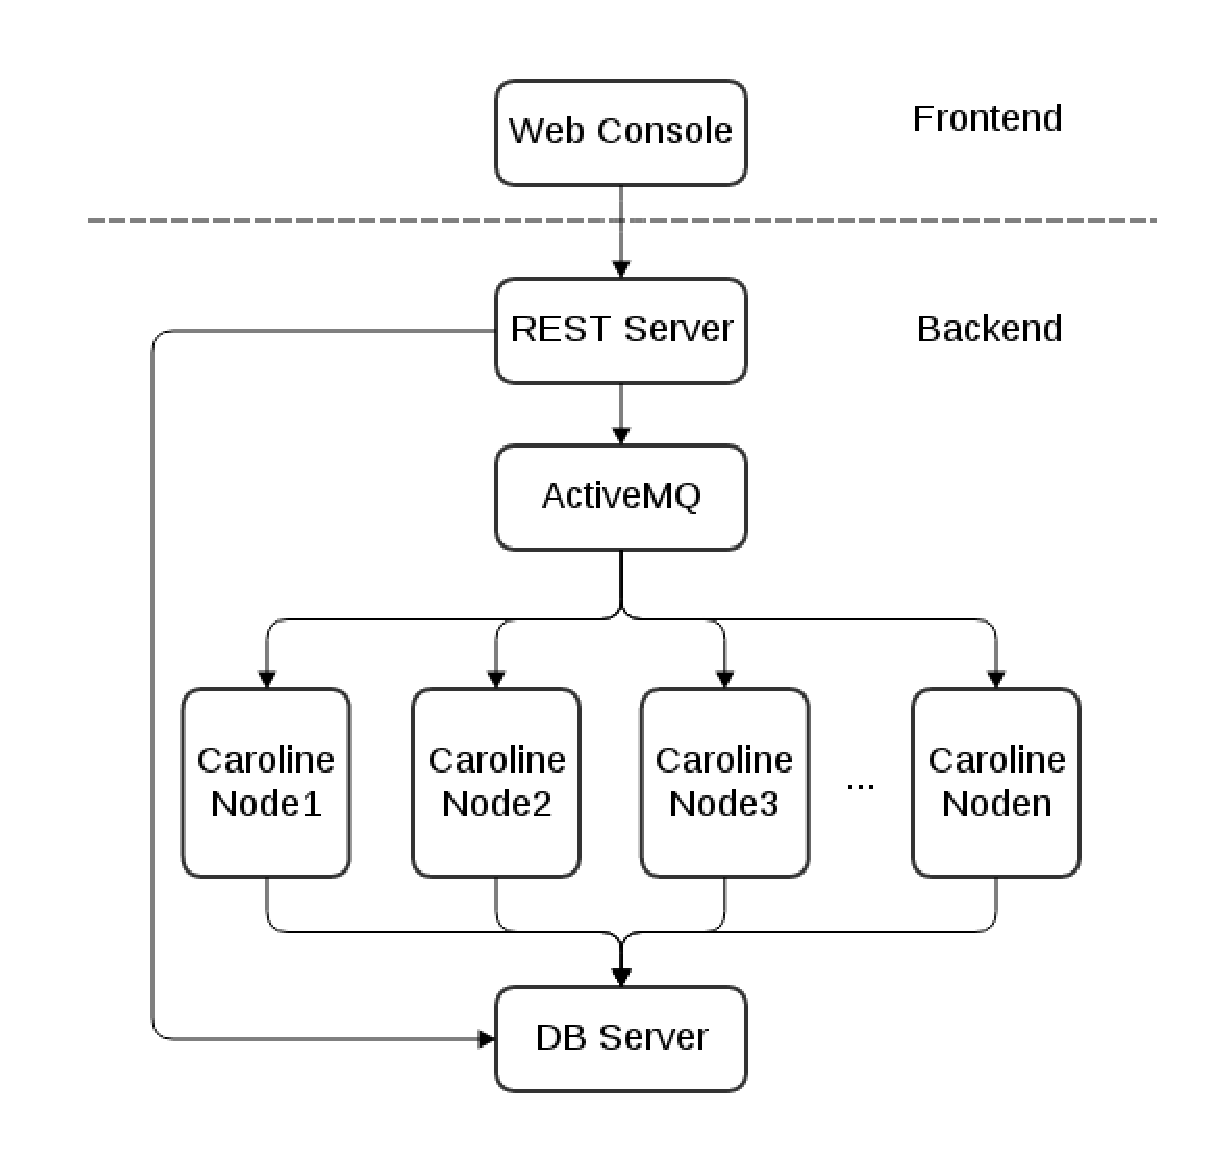
\includegraphics[width=12cm]{fig/revok.eps}
		  \caption{Revok components overview \cite{imgRevokComponents}.}
		  \label{fig:revok-structure}
	\end{figure}
		
	\section{w3af}
	
	Tool w3af (short form for Web Application Attack and Audit Framework) \cite{w3af} is an open source framework used for securing web applications by analyzing and exploiting their vulnerabilities. This cross-platform framework is developed in the Python programming language so it is available for all of the popular operating systems such as Linux, FreeBSD, Mac OS X, Microsoft Windows and others.
	
	w3af can be used via command line but it also provides graphical interface and functionality could be easily extended by using more than 130 available plugins. This framework was started as one man show by Andres Riancho in March 2007, but later (in July 2010) sponsorship and partnership with Rapid7 was announced (which allowed rapid development of this framework).
			
	\section{Wapiti}
	
	Wapiti \cite{Wapiti} is a web application vulnerability scanner using black\-box approach for testing and evaluating web application's security. Wapiti is developed in Python and it supports both GET and POST HTTP methods for discovering possible vulnerabilities. Once the structure mapping of targeted application is finished, Wapiti will try to test payloads to test whether discovered scripts and forms are vulnerable or not.	
	
	Wapiti provides only command line interface so it is not as user friendly as other scanners providing web interface, so it is more suitable for experienced users. Wapiti, like other tested scanners, is completely open source released under GPLv2.0 \cite{GPLv2} license.

		
	\section{ZAP}
	
	ZAP (short for Zed Attack Proxy) \cite{ZAP} is penetration testing tool developed by OWASP foundation \ref{OWASP} and used for finding vulnerabilities in web applications. It provides both passive and active scanners and can be used either for automatic or manual testing. ZAP behaves as intercept proxy and could be used in combination with properly configured web browser to browse pages manually and manipulate all of the traffic coming through.
	
	It is suitable for absolute beginners as well as for skilled testers because it provides very wide range of functionalities. In daemon mode it could also be controlled by powerful REST API \cite{RESTAPI}.
	
	ZAP is one of the most active OWASP projects and it is a part of OWASP flagship project. It is developed in Java and distributed under Apache License v2.0 \cite{APACHEv2}. It was also awarded in recognizing competitions (e.g. second place in the Top Security Tools of 2014 as voted by ToolsWatch.org readers \cite{zap-toolswatch}).
	
	\newpage
	
	\section{Features summary}\label{features}
	
	Each of the tested scanners has its own subset of implemented features. In the table \ref{tab:listOfFeatures} only general features of each scanner are mentioned.
	
	\begin {table}[H]
	\begin{center}
	\bgroup
	\def\arraystretch{1.2}
	\rowcolors{1}{}{lightgray}
	\begin{tabular}{| l | c | c | c | c | c | c | c | r |}
    \hline
	Scanner	& CLI		& GUI 		& WEB		& API		& Report 	 & Log 	& Pause	& Parallel scans \\ \hline
	Arachni	& \cmark	& \xmark	& \cmark	& \cmark	& \cmark	 & \cmark	& \cmark	& \cmark \\
	Revok	& \xmark	& \xmark	& \cmark	& \cmark	& \cmark	 & \cmark	& \xmark	& \cmark \\
	w3af	& \cmark	& \cmark	& \xmark	& \xmark	& \cmark	 & \cmark	& \cmark	&  \xmark \\
	Wapiti	& \cmark	& \xmark	& \xmark	& \xmark	& \cmark	 & \cmark	& \xmark	&  \xmark \\
	ZAP		& \xmark	& \cmark	& \xmark	& \cmark	& \cmark	 & \cmark	& \cmark	&  \xmark \\ \hline			
	\end{tabular}
	\egroup
	\caption{List of implemented features.}
	\label{tab:listOfFeatures} 
	\end{center}
	\end {table}
	
	\subsection{User interface}
	
	Most of the tested scanners have some form of graphical interface (represented by columns GUI and WEB) which can be also used by less experienced users for submitting their tests. Only one of them (Wapiti) has command line interface (column CLI in table above) only.	
	
	\subsection{Reporting and logging}
	 All of the tested scanners are able to create scan report (usually in form of web page) so it is easier for user to check the results of performed scan. These results usually contain also useful hints and recommendations on how to improve security of tested web application. All of tested scanners also provide functionality of logging results to some log files (in form of plain text or formatted for example using JSON \cite{JSON}).
	 
	 \subsection{Remote access and API support}
	Some of the tested scanners (Revok, Arachni and ZAP) provide remote API (REST \cite{RESTAPI} or RPC \cite{RPCAPI}) which can be used for integration these scanners to automated testing workflows like continuous integration testing. The rest of the tested scanners do not support any kind of remote API.
	
	\subsection{Parallel scans and pause functionality}	 
	 Some of the tested scanners are also able to pause running tests and resume them later (represented by column Pause in table \ref{tab:listOfFeatures}). Only two of the tested scanners (Revok and Arachni) are capable to be deployed on multiple nodes and provide parallel scans functionality.
	
\chapter{Testing and evaluation}\label{testing-evaluation}

The selected tools have been used for testing and evaluating possibilities and efficiency of each web application vulnerabilities scanner mentioned in the chapter Analysis of existing solutions \ref{analysis}. Each one of these tools is briefly described bellow. The results of all tested scanners are presented in chapter Results \ref{results}. Installation of each scanner and testing suite is described in appendix \ref{app:installation-and-usage} and arguments, enabled modules and targets used during testing are described in table \ref{tab:resultsWivetDetailed}.

	\section{Testing methodology}\label{testing-methodology}
	
	All tested scanners have been running multiple times with various arguments. In the first run, all of the tested scanners, including Revok, have been tested in default configuration and with all default modules enabled. In the second run, there were only appropriate modules enabled for each attack vector and scanner. These two runs have been compared with each other and only the highest earned score for each vector type and each scanner has been recorded. 
	
	Later testing has been realized using open source CI (continuous integration) testing tool called Jenkins \cite{jenkins}. For both testing suites (WIVET and WAVSEP) have been created jobs which fully automated testing of Revok scanner against these testing suites. Details of Jenkins CI implementation is presented in chapter Jenkins CI tool for Revok \ref{jenkins}.
		
		%\subsection{WASSEC}
		%http://projects.webappsec.org/w/page/13246986/Web%20Application%20Security%20Scanner%20Evaluation%20Criteria
		%\todo{Web Application Security Scanner Evaluation Criteria}

		\subsection{WIVET}\label{wivet}
		
		WIVET \cite{WIVET} (short for Web Input Vector Extractor Teaser) is a benchmarking project that measures how effective is tested scanner in crawling web applications and in finding possibly exploitable input vectors. WIVET project is developed in PHP \footnote{PHP - Hypertext Prepropcessor, popular general-purpose scripting language}, which means that it could be hosted on almost any common hosting (which supports PHP). Deployment and usage of this tool is straightforward and does not require any additional configuration. WIVET itself provides very easy-to-use web interface where you can see actual progress of testing and also the total coverage of each scanner (statistics are bounded to the PHPSESSID\footnote{PHPSESSID - Unique session identificator used by PHP applications to determine different clients.}). Detailed installation and usage of this tool is described in appendix \ref{app:installation-of-wivet}.

		\subsection{WAVSEP}\label{wavsep}
		
		WAVSEP \cite{WAVSEP} (short for Web Application Vulnerability Scanner Evaluation Project) is the evaluation platform which contains a collection of unique web pages. Each of them is vulnerable in different way so the whole framework provides possibility to test various properties of web application scanners. WAVSEP is developed in Java and it uses Tomcat \cite{TOMCAT} application server for running. Detailed installation and usage of this tool is described in appendix \ref{app:installation-of-wavsep}. This project does not contain any kind of evaluation so custom evaluation method has been used (details will be presented in following section).
		
	\section{Evaluation}\label{evaluation}
	
	This section describes steps which have been performed in order to evaluate efficiency and detection accuracy of each class of vulnerabilities using testing suites WIVET and WAVSEP. Specific testing scenarios which have been used for testing and evaluating are mentioned in table \ref{tab:resultsWivetDetailed}.
	
		\subsection{WIVET}

		Each one of tested scanners has been tested first against WIVET \ref{wivet} to determine coverage of each attack vector. WIVET itself is capable to evaluate ability of each scanner to use particular attack vector and also to present the results via its web interface. WIVET includes tests for 56 different attack vectors so it is possible to express the success ratio of each scanner in percentage. WIVET results are presented in chapter \ref{results}, section \ref{wivet-results}. For testing coverage of each scanner has been used WIVET in version 4.
	
		\subsection{WAVSEP}	
	
		WAVSEP is vulnerable web application which contains a collection of unique web pages. The WAVSEP contains 1261 vulnerable pages in total (142 SQLi, 98 XSS, 828 LFI, 115 RFI and 78 other vulnerabilities which are not mentioned in this thesis). Each class of web attacks (SQLi, XSS, LFI, RFI) was tested separately and only dedicated plugins/modules were enabled during these tests. For testing abilities of selected scanners was used WAVSEP in version 1.5.
		
		\subsection{Evaluation using WAVSEP}
		This testing platform provides only links to vulnerable pages and description of each vulnerability but does not provide any way of evaluating the detection accuracy of each scanner. For this reason I have created scripts which helped me to gather links of all vulnerable pages from WAVSEP to the testing database and parse logs of each scanner/attack. I have determined discovered vulnerabilities from these logs and then evaluated the overall detection accuracy. All of these scripts are located on attached DVD in directory \textit{bp-jenkins-scripts} and more complex usage along with dependencies are described in appendix \ref{app:installation-of-wavsep}. Wavsep testing and evaluation of Revok's results have been simplified and transformed to separate Jenkins job. This job was used later for testing Revok's improved testing capabilities (after applying all changes mentioned in chapter Features implementation \ref{features-implementation}).
		
		\subsubsection{Gathering links}			
		The list of the unique URLs for testing pages was generated using script \textit{wavsep-gather-links.sh}. This script is using the same configuration file as the one used by Jenkins scripts (which will be introduced later \ref{jenkins}). This script takes only one parameter from command line -- the name of the vector which it should generate links for (allowed values are: \textit{sql, xss, lfi and rfi}). The rest of the configuration options is located in the shared configuration file which is also used for Jenkins scripts. This script also uses the location of your WAVSEP installation (e.g. \textit{http://localhost:8082/wavsep/}).
		
		\subsubsection{Database initialization}		
		For initializing database was used script \textit{wavsep-init-db.sh} which uses as a parameter the name of the SQL file containing links of vulnerable pages. I have used this database as a reference for evaluating whether the scanner discovered this particular vulnerability or not.
		
		\subsubsection{Log file analysis}				
		Analysis of generated log files from each scanner was performed by running script \textit{wavsep-eval.sh} which takes as an argument the name of the analyzed scanner. It searches for log files in directory \textit{results} and performs analysis of logs which match the name (e.g. \textit{revok-xss.html}, \textit{revok-sql.html} and others).
	
		\subsubsection{Gathering statistics}		
		Script \textit{wavsep-results.sh} was used for the gathering of final statistics, which prints on standard output the information about successfully discovered attacks of each class for each tested scanner.	
		
		
	\subsection{Testing and evaluation using Jenkins}
	
	The continuous integration testing for Revok open source web application scanner has been proposed in section Proposed features \ref{proposed-features} and later implemented and described in section Features implementation \ref{features-implementation}. Jenkins jobs allow fully automated testing of Revok's capabilities and these jobs have been created for both testing suites (WIVET and WAVSEP). Details about them, their configuration and usage is described later in this thesis.
				
	\section{Tested vulnerabilities}\label{testing-vulnerabilities}
	
		In this section there are the tested vulnerabilities presented and possibility of its exploiting is explained.
	
		\subsection{SQLi}

		According to the OWASP \cite{SQLi}, SQL injection (also known as SQLi) is one of the commonly used attacks performed and tested against web (and not only) applications. It consists of insertion SQL \footnote{SQL - Structured Query Language} query via some input vector to the application which causes its execution. SQLi depends on incorrectly sanitized user's input which is used for injection attacker's code into the original query. This attack could lead to revelation of sensitive data stored in application database, allowing data manipulation (update,insert or even delete) and even administration operations can be executed on database.
		
		\subsection{XSS}\label{xss}
		
		The Cross-site Scripting (also known as XSS) is, according to the OWASP \cite{XSS}, another type of remote injection attack which uses injecting of malicious script for exploiting legitimate web site. This attack occurs whenever are the untrusted data received by the application and sent to the victim's web browser without proper escaping or validation (XSS allows executing of malicious script in victim's browser). This attack has very wide range of use and it is very difficult to detect by the victim. As stated by OWASP \cite{XSS-types}, there are three variants of this attack:
		
		\begin{itemize}
			\item Stored XSS 
			\item Reflected XSS
			\item DOM Based XSS
		\end{itemize}
		
		This was the basic classification but it is also possible to divide Cross-site Scripting attacks by accessibility:
		
		\begin{itemize}
			\item Server XSS - occurs when malicious code is included in an HTML response received from the server
			\item Client XSS - occurs when malicious code is used to update the DOM by the Javascript call
		\end{itemize}
		
		Exploiting of these vulnerabilities could be used for accessing victim's sensitive data (e.g. cookies, session tokens and others) and also running malicious script in victim's browser (it could be used for example for updating content of the affected page).
		
			\subsubsection{Non-Persistent XSS}
			It is the most common type of XSS vulnerability because malicious code is not stored anywhere persistently and therefore does not require any additional interaction with any storage system (e. g. database system). For exploiting this vulnerability any user input which is not properly sanitized could be used.
		
			\subsubsection{Persistent XSS}
			This type of XSS attack is similar to the previous one but there is one difference - malicious code is stored persistently on the server (in database, files or any other resource providing storage) and can be exploited multiple times with every refresh of infected page.
		
			\subsubsection{DOM based XSS}
			This kind of attack is performed by changing DOM on client side without any interaction with server so there is no way how to check if client was compromised or not.

		\subsection{LFI and Path traversal}
		
		According to the OWASP \cite{LFI}, Local File Inclusion (also known as LFI) is the vulnerability, that allows the attacker to include files that are already present in the system (unlike Remote file inclusion which will be mentioned later in section RFI \ref{RFI}) to an application via the web browser. This vulnerability occurs when page does not use properly validated and sanitized input. This attack can be used for revealing sensitive data from files present on the system (e.g. configs, files containing passwords and others). This vulnerability is commonly exploited in PHP applications, but can be found also in other technologies (e.g. ASP, JSP).
		
		This vulnerability also allows to use another attack called Path or Directory traversal. Principle of this attack is in exploiting page includes (the same way as in LFI) so an attacker would be able to access files and directories which are not present in the web folders \cite{Path-traversal}.
		
		\subsection{RFI}\label{RFI}
		
		The Remote file Inclusion (also known as RFI) is very similar to the Local File Inclusion vulnerability. The difference between these two vulnerabilities is in including remote files (files hosted on different server) instead of the local ones like in LFI \cite{RFI}.
		
	\section{Approaches commonly used to detect vulnerabilities}\label{approaches}
	
		This section contains brief description of used approaches for detecting each of all mentioned vulnerabilities in web applications.
	
		\subsection{SQLi}

		SQL Injection is still a common web application vulnerability and according to the OWASP Top10 it is the most exploited vulnerability ever. Exploiting an SQL injection is nowadays very easy thanks to automated tools specialized on this kind of vulnerability such as SQLMap \cite{SQLMAP} or SQLNinja \cite{SQLNINJA}. All of them are using set of already predefined payloads and they are trying to inject the same set of payloads to the web application. There are 6 basic payload types used for exploiting SQL injection according to the Arne Swinnen \cite{AutomatedSQLi}:
		
		\begin{itemize}
			\item boolean-based blind
			\item time-based blind
			\item error-based
			\item UNION query
			\item stacked queries
			\item out-of-band queries
		\end{itemize}
		
		
		All of these payload types will be briefly described bellow. More details about these payloads and examples are above the scope of this thesis.
		
			\subsubsection{Boolean-based blind method}
			This method is based on injecting payloads (boolean subquery returning true) which leads to altering the original query and returning different content which was not originally requested.
		
			\subsubsection{Time-based blind method}
			This method is based on injecting payload which causes delay on database server and slows down the speed of the whole application in return.
		
			\subsubsection{Error-based method}		
			This method is using payloads to break the original SQL request and force the database server to generate SQL error presented back to the client.
		
			\subsubsection{UNION query}
			This method is using SQL command UNION for merging results from multiple tables and printing information which was not originally supposed to be returned to the client.
		
			\subsubsection{Stacked queries}
			Method very similar to the UNION query method using multiple queries stacked together.
		
			\subsubsection{Out-of-band queries}			
			This payload method can use for example a file which could be executed inside the web server directory.
		
		\subsection{XSS}		
		Cross-site scripting are attacks where an attacker is able to get control of victim's web browser and use it for executing malicious script (usually in the form of Javascript code). According to the OWASP Top10 it is the third most exploited vulnerability these times. As already mentioned in previous section \ref{xss} there are 3 types of XSS attacks:
		
		\begin{itemize}
			\item Non-Persistent attack (also known as Reflected XSS)
			\item Persistent attack
			\item DOM based attack
		\end{itemize}
		
		There are mainly three kind of approaches for detecting XSS vulnerabilities and they are as following:
		\begin{itemize}
			\item Static analysis
			\item Dynamic analysis
			\item Combination of static and dynamic analysis
		\end{itemize}
		
			Some of the approaches will be briefly described bellow but this topic is too complex to be covered in this thesis. For more details about approaches for detecting XSS please refer to master thesis Approaches to detect SQL injection and XSS in web applications created by Abhishek Kumar Baranwal \cite{thesisApproaches}.
		
			\subsubsection{Static analysis approach}\label{approach-xss-static}
			
			There are many types of static analysis used for detecting XSS vulnerability in web application according to the Abhishek Kumar Baranwal's thesis \cite{thesisApproaches}:
			
			\begin{itemize}
				\item Bounded Model Checking
				\item Analysis of String
				\item Software Testing Approaches
				\item Taint Propagation Approach
				\item Using Untrusted Scripts
			\end{itemize}
			
			\subsubsection{Dynamic analysis approach}\label{approach-xss-dynamic}
			
			\begin{itemize}
				\item Syntactical Structure Approach
				\item Interpreter-based Approaches
				\item Browser-Enforced Embedded Policies Approach
				\item Proxy-based Approach
			\end{itemize}	
			
			\subsubsection{Static and Dynamic Analysis Approach}\label{approach-xss-static-and-dynamic}	
			
			\begin{itemize}
				\item Lattice-based Approach
			\end{itemize}
		
		\subsection{Path traversal and LFI}
		This vulnerability is the result of insufficient validation and sanitization of browser input from users. Path traversal (also known as directory traversal) vulnerability can be located either in web server implementation or application itself and this vulnerability can exist in a variety of programming languages (it is not limited only to PHP and web applications).
		
		Attackers exploiting this vulnerability send malicious URL to the server which instructs web server to return specific files. Attacker has to find URL which can be modified to retrieve the file from the server. The `../` sequence is commonly used for exploiting this vulnerability which basically instructs the web server to retrieve file from parent directory.
		
		Local File Inclusion attack is very similar to the Path Traversal attack. The difference between them is that for exploiting LFI attacker uses files which are located on the targeted server. The most often used file on Linux systems is \textit{/etc/passwd} because attacker can be absolutely sure that it exists and it is accessible and readable by the web server. Attacker can use this vulnerability for retrieving of any file located on targeted server (any file which can be accessed by the user running web server or another exploited service).
		
		\subsection{RFI}
		Remote File Inclusion vulnerability is very similar to the LFI. The only difference between them is that in this case attacker uses file which is not stored locally but it is located on remote server (usually on server controller by attacker). Attacker's goal is to include remote file and force web server or hosted application to execute this included file. Exploiting this vulnerability is commonly used for uploading malicious scripts to victim server (very often used are tiny scripts which provide remote shell support or FTP access so attacker can easily upload new files and continue with exploiting application/server).
	
	\section{Results}\label{results}

	This sections presents WIVET and WAVSEP results of each tested scanner. Used testing methodology and information how to interpret results was already described in the chapter Testing and evaluation \ref{testing-evaluation}. Specific testing scenarios used for testing scanners are mentioned in table \ref{tab:resultsWivetDetailed}.

	\subsection{WIVET results}\label{wivet-results}	
	
	All of the scanners has been tested against WIVET testing suite and results of evaluating ability of each scanner to use various attack vectors are mentioned in table \ref{tab:resultsWivet}. All of the tested scanners were tested multiple times with different modules enabled and only the highest score was recorded for comparison.
	
	\begin {table}[H]
	\begin{center}
	\bgroup
	\def\arraystretch{1.2}
	\rowcolors{1}{}{lightgray}
	\begin{tabular}{| l | ccccc |}
    \hline
	 & Arachni	& Revok & w3af	& Wapiti	& ZAP \\ \hline
	Total coverage & 96\%		& 0\%	& 16\%	& 44\%		& 69\%	\\ \hline
	\end{tabular}
	\egroup
	\caption{WIVET results}
	\label{tab:resultsWivet} 
	\end{center}
	\end {table}
	
	Results of testing scanners against WIVET testing suite with information about used modules are mentioned in table \ref{tab:resultsWivetDetailed}.
	
	\begin {table}[H]
	\begin{center}
	\bgroup
	\def\arraystretch{1.2}
	\rowcolors{1}{}{lightgray}
	\begin{tabular}{| l | l | r |}
    \hline
	Scanner & Enabled modules	& Coverage  \\ \hline
	Wapiti	& xss				& 44\%		\\ \hline
	w3af	& web-spider		& 12\%		\\ \hline
	w3af	& web-spider, digit-sum & 16\%	\\ \hline
	Revok	& all				& 0\%		\\ \hline
	Arachni	& trainer, audit-links, audit-forms	& 96\% \\ \hline
	ZAP		& basic				& 10\%		\\ \hline
	ZAP		& subtree			& 16\%		\\ \hline
	ZAP		& subtree, ajax		& 69\%		\\ \hline	
	\end{tabular}
	\egroup
	\caption{WIVET results according to enabled modules}
	\label{tab:resultsWivetDetailed} 
	\end{center}
	\end {table}	
	
	
	For more detailed WIVET results please refer to the appendix \ref{app:detailedResultsWIVET} where you can find the list of all tested vectors and corresponding results for each of tested scanners.
	
	\subsection{WAVSEP results}\label{wavsep-results}
	
	All of the tested scanners have also been tested against WAVSEP testing suite and results of each scanner are presented in table \ref{tab:resultsWavsep}. Only relevant modules of each scanner were used for testing each class of vulnerability. 
	
	\begin {table}[H]
	\begin{center}
	\bgroup
	\def\arraystretch{1.2}
	\rowcolors{1}{}{lightgray}
	\begin{tabular}{| l | ccccc |}
    \hline
	Vulnerability		& Arachni		& Revok 	& w3af		& Wapiti		& ZAP \\ \hline
	SQLi				& 100\%			& 32\%		& 35\%		& 100\%			& 100\% \\ \hline
	XSS					& 90\%			& 88\%		& 37\%		& 66\%			& 100\% \\ \hline
	LFI					& 100\%			& 0\%		& 57\%		& 51\%			& 75\% \\ \hline
	RFI					& 100\%			& 31\%		& 16\%		& 57\%			& 100\%	 \\ \hline
	Total score			& 97.5\%		& 37\%		& 36.2\%	& 68.5\%		& 93.7\% \\ \hline
	\end{tabular}
	\egroup
	\caption{WAVSEP results}
	\label{tab:resultsWavsep} 
	\end{center}
	\end {table}
	
	\subsection{Results overview}
	
	The highest score reached by all of the tested scanners is mentioned in table \ref{tab:resultsOverview}. According to this table it is evident that the Arachni scanner performed the best with total score 96.8\%, followed by ZAP which reached score 81.35\%. The difference between the 2nd (ZAP) and 3rd position (Wapiti) is relatively big because Wapiti reached only 56.25\%. The rest of the tested scanners reached even lower score (scanner w3af reached 26.1\% and Revok only 18.5\%).
	
	\begin {table}[H]
	\begin{center}
	\bgroup
	\def\arraystretch{1.2}
	\rowcolors{1}{}{lightgray}
	\begin{tabular}{| l | ccccc |}
    \hline
	 				& Arachni	& Revok 	& w3af		& Wapiti	& ZAP		\\ \hline
	WIVET			& 96\%		& 0\%		& 16\%		& 44\%		& 69\%		\\ \hline
	WAVSEP			& 97.5\%	& 37\%		& 36.2\%	& 68.5\%	& 93.7\% 	\\ \hline
	Total score 	& 96.8\%	& 18.5\%	& 26.1\%	& 56.25\%	& 81.35\%	\\ \hline
	\end{tabular}
	\egroup
	\caption{Results overview}
	\label{tab:resultsOverview} 
	\end{center}
	\end {table}


\chapter{Missing features in Revok}\label{missing-features}

	\section{Revok's results evaluation}

	According to the results of each scanner mentioned in the previous section, Revok is not the most effective and powerful scanner on the list of tested scanners although it performed well. As stated in table \ref{tab:resultsWivet}, Revok scored with result 0\% only in WIVET test and it did not even passed basic tests.
	
	As stated in table \ref{tab:resultsWavsep} Revok is the most effective in finding XSS vulnerabilities, on the second place was discovering SQL injection and Remote File Inclusion vulnerabilities. It is also apparent, that Revok has problems with detection of Local File Inclusion and Path Traversal vulnerabilities although it already contains dedicated plugin for finding Path Traversal vulnerabilities.
	
	\section{Proposed features}\label{proposed-features}
	
	For testing new features implementation it is necessary to establish a testing environment which allows the possibility of an automated testing of efficiency and reliability of the new implemented features. This automated testing environment can be also used for ensuring that no regressive problem will be integrated to the new version of the Revok. It also means that the possibility that regressive problem will be integrated to the next release during the development cycle. For this purpose Jenkins CI Continuous Integration project has been used. More information about the configuration, host topology and usage of the Jenkins CI testing environment used in this specific project is presented in the following section Features implementation \ref{features-implementation}.
	
		\subsection{Enhancement of web crawler}	
		
		The another proposed change/feature is to identify the problem causing the zero score for Revok in WIVET tests, develop fix for this problem, create pull request and inform developers and community where and what was the problem (ideally in form of creating issue and pull request afterwards). 
		
		\subsection{Improve LFI detection}
		
		Enhance the testing and detection capability of already existing Path Traversal module and implement/add new checks for finding Local File Inclusion vulnerabilities. 
		

\chapter{Features implementation}\label{features-implementation}

	In this chapter will be presented new features and their implementation to the open source scanner Revok which was proposed earlier in section Proposed features \ref{proposed-features}.

	\section{Enhancement of web crawler}
	
	First proposed change was enhancing testing capability of Revok's web crawler to improve results  in WIVET testing.
	
		\subsection{Problem with relative links handling}\label{crawler-problem-1}
	
		As I already mentioned in previous section, Revok has obvious problems with WIVET testing suite because it scored only 0\%. After some research I've discovered that this poor score was caused by the lacking capability of handling html base tag during Revok's crawlering phase. 
	
		Revok was not able to handle relative links in case that there is HTML base tag present on the scanned page. This issue is not actually caused by Revok itself because Revok only uses project PhantomJS  \cite{phantomjs} for the whole process of analyzing / crawling the targeted page. PhantomJS is scripted headless browser based on Webkit which provides full web stack (including Javascript). There is already known issue \cite{phantomJSissue} with handling relative URLs in PhantomJS but this problem is still not resolved.
	
		Due to this bug, Revok was not able to resolve relative links properly and it led to 0\% score reached in WIVET testing. The problem is that WIVET uses multiple frames on one page and there is base tag located in one of them. Although Revok was able to identify all links on scanned paged properly it was not able to combine the address stored in base tag with the relative links found on page. Because of this, Revok did not even reach these pages - server returned \textit{Error not found} instead.	
	
		This problem has been already reported to the Revok team (on their original GitHub repository \cite{Revok}). Issue request has been created with detailed description of this problem \cite{GitHubIssue1}. This lacking capability caused problems with proper web crawling, more specifically with the relative link handling. Possible fix/workaround for this issue has been developed and also introduced to the Revok's developers and community. Pull request \cite{GitHubPullRequest1} has been created for this purpose. Patch containing this fix/workaround is also located on attached DVD \ref{app:cd}.
	
		\subsection{Problem with multiple events on single page}\label{crawler-problem-2}
		
		Fixing problems with handling relative links mentioned in previous section improved WIVET testing coverage, but only to 19\%. After this change Revok was able to handle basic attack vector like redirects. It was also able to handle some click and mouse events but not on all of them. 
		
		There was an implementation of basic method called \textit{scanOthers} in web crawler module \textit{webcrawler.js} which was supposed to perform basic click events on elements \textit{li} and \textit{span}. This implementation relied on fact that there is only one event with click event binded at the same time on single page. Web crawler module is also using jQuery \cite{jquery} javascript library for easier orientation on scanned page (it allows easier DOM manipulation and provides powerful DOM selectors). 
		
		The base functionality of \textit{scanOthers} method was to match all occurences of \textit{li} and \textit{span} elements and perform delayed click on each of them. The problem with this approach was that the first executed click event triggers redirect event and the whole page was redirected to different page. Redirect causes that none of the rest of delayed click events will be processed anymore.
		
		There is one limitation which prevents from implementing easy and straightforward solution of this problem. Every action performed on scanned page using PhantomJS is sandboxed (method \textit{evalute} which takes callback function as an argument). It also means that jQuery framework can be only used inside this sandboxed function and it is problematic to pass arguments to this function and return multiple values from it.
		
		This problem has also already been reported to the Revok team and issue request for this problem has already been created \cite{GitHubIssue2}.
		
		I have developed possible solution for this problem and I already pushed this change to my forked repository. I have implemented method called \textit{scanEvents} which is able to go through all elements specified in array \textit{objectSelectors} and perform all events specified in array \textit{events}. Supported elements currently are: \textit{div}, \textit{li} and \textit{span}, but it is possible to add other elements as well. There are also new events supported in this implementation:
		
		\begin{itemize}
			\item click - event occurs when the user clicks on an element
			\item mouseout - event occurs when the mouse pointer is moved out of an element
			\item mouseover - event occurs when the mouse pointer is moved onto an element
			\item mousedown - event occurs when the user press' a mouse button over an element
		\end{itemize}
		
	This method uses workaround for identifying all selected elements with ID before triggering events even start. For this purpose is every element which should be tested (it means that events should be triggered on this element) marked with unique ID (in case that it does not have ID already). Then we are able to track down which element (by ID) was already tested and which was not and we can go through all of them creating sandbox for triggering every single event (it will not affect other events).

	Pull request \cite{GitHubPullRequest1} has been created for this purpose. Patch containing this fix/workaround is also located on attached DVD \ref{app:cd}.

	\section{Improve LFI detection}
	
	The second proposed change was improving capability of detecting Local file inclusion vulnerability in WAVSEP tests.
	
		\subsection{Problem with limited list of entry points}\label{lfi-problem-1}
		
		The Revok scanner uses only predefined and very limited list of entry points for testing both Local and Remote file inclusion vulnerabilities. There is only one module present in Revok scanner which is responsible for scanning all three vulnerabilities (LFI, RFI and Path traversal) and it is called \textit{path\_traversal} module (stored in file \textit{path\_traversal.rb}). Revok provides possibility to select which modules will be used for requested scan so this module can be easily tested separately to ensure that results will not be influenced by another modules.
		
		This module contains a list (it is an array \textit{f\_name}) of predefined entry points and only these entry points are tested and evaluated in this module. The list of these predefined entry points is as following: \textit{doc, file, f, page, p, dir, filename, fname}.
		
		The problem in this approach is that WAVSEP uses different entry point (namely \textit{target}) so Revok was not able to test file inclusion attacks only with \textit{path\_traversal} module enabled. Revok is able to discover some RFI vulnerabilities with XSS modules enabled but it does not work with Local file inclusion and Path traversal vulnerabilities.
		
		Solution of this problem is to add entry point used by WAVSEP to list of predefined entry points which uses Revok's \textit{path\_traversal} module. Issue request \cite{GitHubIssue3} has been created with suggested workaround which can be used as temporary solution.
		
		\subsection{Problem with stability of WAVSEP testing suite}\label{lfi-problem-2}
		
		During testing Revok's ability to detect Local file inclusion vulnerabilities using WAVSEP testing suite I have experienced various problems with stability of the whole testing suite. When I was testing some LFI pages, which are part of the WAVSEP testing suite, Tomcat server stopped responding. The problem occurred only when all LFI pages were tested in one scan. I have also tried to separate LFI pages to smaller groups divided by used protocol and expected return value (WAVSEP itself provides this separation using different index files for each combination of used protocol and expected return code) and it worked without any problem. This problem occurred also when I was testing LFI testing capability of other open source scanners mentioned in this thesis.
		
		This problem with WAVSEP was already reported by Isaac Dawson \cite{OWASPIssue1} and Tasos Laskos \cite{OWASPIssue2}.
		
		The default behavior of the crawler module implemented in Revok scanner is to return only the target URL when remote server stops responding. This, with combination of previously mentioned problem, led to 0\% testing score in WAVSEP tests.
		
		Solution of this problem is to test each combination of tested protocol and expected return value separately and then merge these results together to get the final score. WAVSEP contains tests for 2 HTTP methods (POST and GET) and following HTTP responses:
		
		\begin{itemize}
			\item Errorneous HTTP 500 Responses
			\item Errorneous HTTP 404 Responses
			\item Errorneous HTTP 200 Responses
			\item HTTP 302 Redirect Responses
			\item HTTP 200 Responses With Differentiation
			\item HTTP 200 Responses with Default File on Error
		\end{itemize}		
		

	\section{Jenkins CI tool for Revok}\label{jenkins}
	
		For automated testing of new Revok features implementation has been used open source continuous integration tool Jenkins \cite{jenkins}. Jenkins  is an open source continuous integration tool developed in Java. This project is licensed under MIT \cite{MIT} license and it was originally forked from project Hudson. This tool has been chosen for this purpose because it offers many advantages such as:
		
		\begin{itemize}
			\item Easy installation (can be installed from rpm or via yum package manager)
			\item Easy configuration (the entire Jenkins can be configured via web user interface)
			\item Change set support (Jenkins can generate a list of changes between builds)
			\item Distributed builds (builds can be distributed to multiple nodes)
			\item Plugin support (Jenkins can be extended via many 3rd party plugins)
		\end{itemize}
		
		\subsection{What is continuous integration}
			
		Continuous integration (also known as CI) is according to the TechTarget definition \cite{CI-definition} \emph{"software engineering practice in which isolated changes are immediately tested and reported on when they are added to a larger code base. The goal of CI is to provide rapid feedback so that if a detect is introduced into the code base, it can be identified and corrected as soon as possible"}.
		
		\subsection{Jenkins job for testing Revok against WIVET}
		
		For testing and evaluating Revok against WIVET testing suite Jenkins job called \textit{Wivet-testing-suite} has been created. Configuration file for this job in form of XML is located on attached DVD \ref{app:cd}. Job is parameterized and can be executed in production and testing mode. The difference between these two modes is in the path of the Revok repository (these two paths are stored in configuration file for Jenkins scripts and can be adjusted). This job is also configured to store all log and result files from latest builds on Jenkins master so they can be analyzed later manually. Job itself consists from calling 3 separate scripts.
		
			\subsubsection{Script wivet-start.sh}
			
			This script is responsible for installing any necessary dependencies needed for running Revok and WIVET test suite. It also creates necessary folders with proper rights, clones both tools from paths specified in configuration file to destinations and ensures that service httpd is started and running prior executing tests.
			
			\subsubsection{Script wivet-test.sh}
			
			This script is used for testing Revok against WIVET test suite. It ensures that httpd service is running and also that all directories and tools created or cloned are on the right places. 
			Testing against WIVET does not require having all Revok's services running because it is needed to test only web crawler module. Revok uses mitmdump \cite{mitmdump} as intercept proxy for analyzing the whole communication between web crawler module and the target so this script ensures that this proxy is started prior the crawler itself. After this operation PhantomJS process is started with proper arguments, it performs initialization of web crawler module and starts the scan. This script also ensures that once scan finishes both, mitmdump and PhantomJS processes are terminated.
			
			\subsubsection{Script wivet-stop.sh}
			
			Last script, which is used for testing and evaluating Revok's capability using WIVET in Jekins, is responsible for stopping all services that are not needed anymore, cleaning all files created only for testing purposes and also evaluating test results from statistic files generated by WIVET suite. The example of results generated by this Jenkins job is presented on screenshot \ref{fig:screen-wivet}.
		
		\subsection{Jenkins job for testing against WAVSEP}
		
For testing and evaluating Revok against WAVSEP testing suite very similar Jenkins job to the previous one called \textit{Wavsep-testing-suite} has been created. Configuration file for this job in form of XML is located on attached DVD \ref{app:cd}. Job is parameterized and can be executed in production and testing mode. The difference between them is the same as is in the job mentioned earlier. There is one additional parameter which can be used for customizing this job. This parameter is specifying attack vectors which should be tested. Allowed choices are: \textit{all, sql, xss, lfi-partially}. The last one represents the workaround mentioned earlier in section \ref{lfi-problem-2}. This job is also configured to store all log and result files from latest builds on Jenkins master so they can be analyzed later manually. Job itself also consists from calling 3 separate scripts.
	
			\subsubsection{Script wavsep-start.sh}
			
			This script is responsible for installing all needed dependencies for running Revok and WAVSEP test suite. It also creates necessary folders with proper rights, clones both tools from paths specified in configuration file to destinations and ensures that service tomcat \cite{TOMCAT} is started and running prior executing tests.			
			
			\subsubsection{Script wavsep-test.sh}
			
			WAVSEP testing suite is more complex (in sense of preparing test environment) than WIVET one. For testing internal modules it is needed to start all Revok services and not only the two as in case of WIVET. This script ensures that all Revok's services are started and running properly and then requests all scans of attack vectors specified at the beginning. Requesting scans is done via using REST API which Revok provides (using specifically crafted PUT request with corresponding arguments).
			
			\subsubsection{Script wavsep-stop.sh}
			
			This script is responsible for cleaning all testing files and stopping services that are not needed anymore. It is also responsible for evaluating test results of every attack vector enabled and for printing statistics. The example of results generated by this Jenkins job is presented on screenshot \ref{fig:screen-wavsep}.
			
		\subsection{Results after features implementation}		
		
		In this subsection screenshots of Jenkins job containing results for each of used testing suites are presented. The results mentioned below were reached after applying all implemented changes proposed in section \ref{proposed-features} and implemented in section \ref{features-implementation}.
		
		\begin{figure}[h!]
		  \centering
		  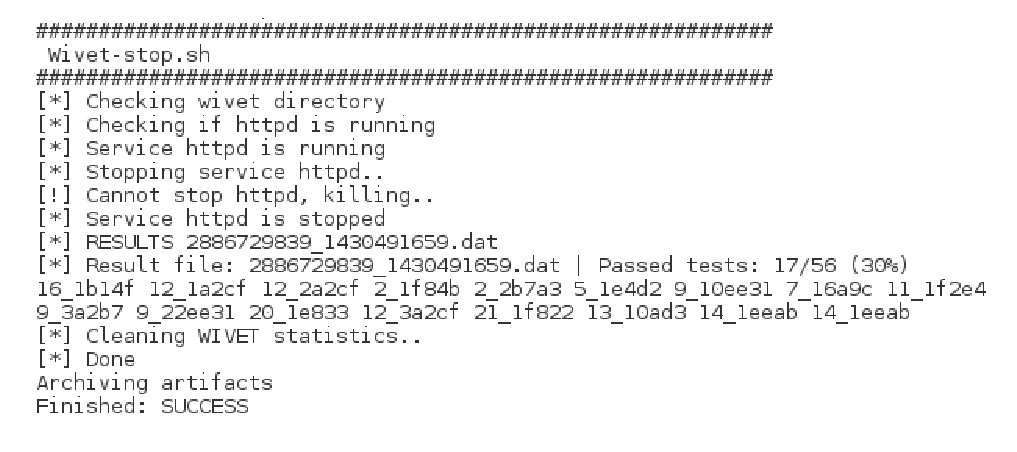
\includegraphics[width=13cm]{fig/jenkins_wivet.eps}
		  \caption{Results of WIVET Jenkins job}
		  \label{fig:screen-wivet}
		\end{figure}
	
		\begin{figure}[h!]
		  \centering
		  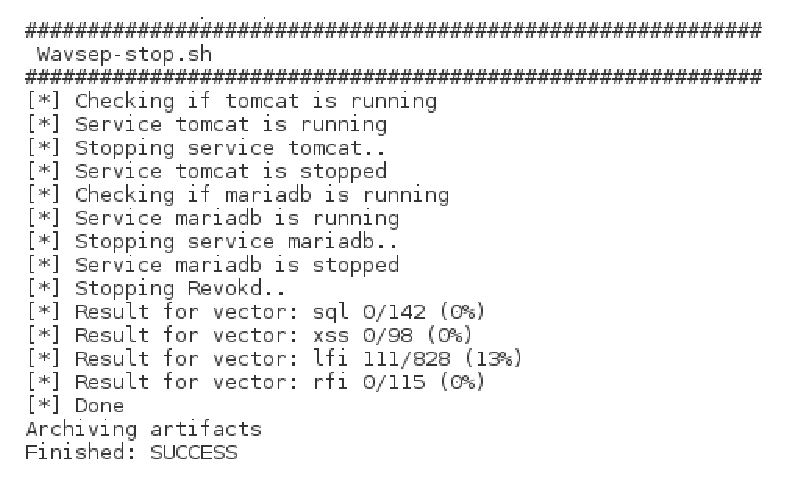
\includegraphics[width=13cm]{fig/jenkins_wavsep.eps}
		  \caption{Results of WAVSEP Jenkins job}
		  \label{fig:screen-wavsep}
		\end{figure}
			
\chapter{Conclusion}\label{conclusion}

		The goal of this thesis was to study, analyze and compare implementation and vulnerability detection capabilities of selected open source scanners. Based on this analysis, the next step was to propose and implement new features or extend the functionality of already existing ones in open source scanner Revok.
		
		This goal has been successfully achieved and detection capabilities of Revok have been extended. After applying all patches mentioned in section \ref{features-implementation} Revok was able to reach \textbf{30\%} testing coverage in WIVET and \textbf{13\%} in WAVSEP LFI testing which is considerably better than the previous 0\% coverage reached in both suites. Continuous integration environment based on open source tool Jenkins has been created and successfully tested, and all bugs and issues discovered during the progress on this thesis have been already reported back to the Revok community.
	
	\section{Future development}
			
	Revok has been recently open sourced, which allowed contribution also from developers and users outside of Red Hat. That definitely helped a lot with improving functionality of this scanner (either in form of creating issue requests or pull requests). There are still plenty of ways of how to improve vulnerability detection (e.g. implementing detection of non-discovered attack vectors in WIVET \ref{tab:extended2}) and Revok has the potential to be more used and become more powerful in detecting vulnerabilities in web applications. 
	However, there are open source projects which already provide detection capabilities with much better results. They are usually supported by already existing large communities (development of some of them is funded by sponsors) so it will be very hard for Revok to compete with such mature projects.

% I am potato!
%=========================================================================
